\section{Основные результаты}
\begin{Lemma}
Пусть даны:(1)единичная окружность с центром в точке O;(2)две хорды, пересекающиеся в точке K и (3) координаты начал и концов хорд - A($\cos\alpha,\sin\alpha$), B($\cos\beta,\sin\beta$), C($\cos\gamma,\sin\gamma$), D($\cos\delta,\sin\delta$)(см. рис. 1).
\begin{figure}[h]
\center{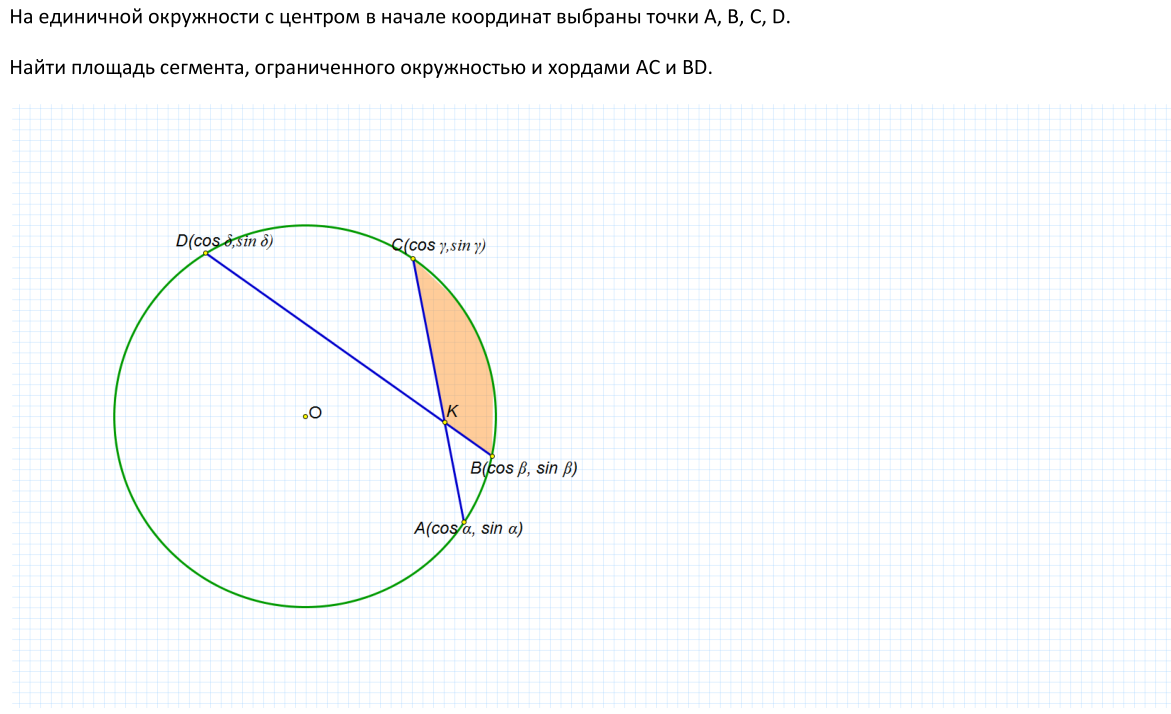
\includegraphics[width=1\linewidth]{prob_1} \\Рис. 1}
\end{figure}
\parТогда площадь фигуры CKB по формуле:
$$S_{BCK}=S_{\triangle BCK}+S_{BC}$$
\end{Lemma}
\proofname
\parВведём обозначения:
$$A = \sin \alpha-\sin\gamma$$
$$B = \cos \alpha-\sin\gamma$$
$$C = \sin \delta-\sin\beta$$
$$D = \cos \delta-\cos\beta$$
$$E = \sin \beta-\sin\gamma$$
$$F = \cos \beta-\cos\gamma$$
$$M = {(EDB + AD\cos \gamma - CB\cos \beta) \over (AD - CB)}$$
$$p = {1\over 2}(\sqrt{F^2-E^2} + |\cos\beta+\cos\gamma-2M|\sqrt{(1+({C\over D})^2})$$
$$p_{\triangle BCO} = {1\over 2}(2+\sqrt{F^2-E^2})$$
$$S_{\triangle BCO} = \sqrt{p_{\triangle BCO}{(p_{\triangle BCO}-1)}^2(p_{\triangle BCO}-\sqrt{F^2-E^2})}$$
Таким образом:
$$S_{\triangle BCK} = \sqrt{p(p-\sqrt{F^2-E^2})(p-|\cos\beta-M|\sqrt{(1+({C\over D})^2)})(p-|\cos\gamma-M|\sqrt{(1+({C\over D})^2)})}$$
$$S_{BC} = R^2\arcsin{(\frac{c}{2R})}-\frac{c}{4}\sqrt{4R^2-c^2},$$ где $R-\;$радиус окружности.
\begin{Theorem}
Пусть дан бесконечный положительный ряд $P=\sum_{i=1}^\infty{s(D_i)\cdot f(\ell(\xi_i))}$. Тогда $\forall\epsilon_1>0\;\exists N(\epsilon_1)$, что при $i>N$
$$\Big\vert\sum_{i=N+1}^\infty{s(D_i)\cdot f(\ell(\xi_i))}\Big\vert<\epsilon_1$$
\end{Theorem}
\proofname
\parСм. раздел 6.1
\begin{Theorem}
Пусть даны два конечных положительных ряда $P_N$ и $Q_N$ такие, что:
$$P_N=\sum_{i=1}^N{s(D_i)\cdot f(\zeta_i)},\;Q_N=\sum_{i=1}^N{s(D_i)\cdot f(R_i)}$$
где $\zeta_i\in D_i$ - произвольное
\parТогда существует такое $\epsilon_2>0$, что выполнено следующее:
$$|P_N-Q_N|<\epsilon_2$$
\end{Theorem}
\proofname
\parСм. раздел 6.2
\begin{Corollary}
Общая погрешность $\epsilon$ алгоритма решения поставленной задачи равна:$$\epsilon=\epsilon_1+\epsilon_2$$
\end{Corollary}